\documentclass{article}
\usepackage{tikz}
\usepackage{geometry}
\usepackage{luatexja}
\usepackage{pgffor}
\usepackage[dvipsnames]{xcolor}
\renewcommand{\kanjifamilydefault}{\gtdefault}
\renewcommand{\familydefault}{\sfdefault}

\newcommand{\docpaperwidth}{2.65cm}
\newcommand{\docpaperheight}{3.95cm}

\geometry{
  papersize={\docpaperwidth,\docpaperheight},
  margin=0cm,
  ignoreall=true
}

\setlength{\parindent}{0cm}
\usetikzlibrary{calc}

\begin{document}
  \center
  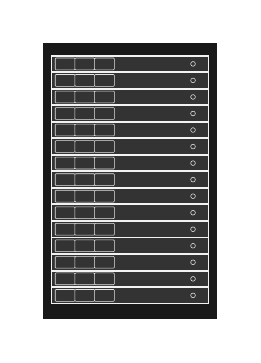
\begin{tikzpicture}
    \path [use as bounding box]
      (-2mm, -2mm) rectangle (24mm, 37mm);

    \newcommand{\svrrack}{(0, 0) rectangle (22mm, 35mm)}
    \newcommand{\svrframe}{(0, 0) rectangle (20mm, 2mm)}
    \newcommand{\svrswa}{(18mm, 1mm) circle [radius=0.3mm]}
    \newcommand{\svrswb}{
      foreach \dx in { 0.5mm, 3mm, 5.5mm } {
        [rounded corners=0.1mm]
        (0 + \dx, 0.25mm) rectangle
        (2.5mm + \dx, 1.75mm)
      }
    }

    \path[fill=black!90!white] \svrrack;
    \foreach \yd in { 0, 2.1,...,30 } {
      \path[fill=black!80!white,
        draw=white!95!black,
        xshift=1mm, yshift=2mm + \yd mm] \svrframe;
      \path[draw=white!90!black,
        xshift=1mm, yshift=2mm + \yd mm,
        very thin] \svrswa;
      \path[draw=white!90!black,
        xshift=1mm, yshift=2mm + \yd mm,
        very thin] \svrswb;
    }
  \end{tikzpicture} 
\end{document}
% vi: se ts=2 sw=2 et:
